\documentclass[12pt,a4paper]{article}
\usepackage[utf8]{inputenc}
\usepackage[T1]{fontenc}
\usepackage[spanish]{babel}
\usepackage[margin=2.5cm]{geometry}
\usepackage{setspace}
\usepackage{parskip}
\usepackage{booktabs}
\usepackage{array}
\usepackage{graphicx}
\usepackage{amsmath}
\usepackage{tikz}
\usetikzlibrary{arrows.meta, positioning, calc}

\tikzset{
    bloque/.style={
        rectangle, rounded corners=4pt,
        draw=black!70, line width=1pt,
        minimum width=8cm,
        text width=7.5cm,
        align=center,
        inner sep=8pt,
        font=\small
    },
    flecha/.style={-Stealth, line width=1pt}
}

\begin{document}

\onehalfspacing

% ---------------------------------------------------------------
% PORTADA
% ---------------------------------------------------------------
\begin{titlepage}
    \centering
    \vspace*{3cm}

    {\Large \textbf{Universidad de Guadalajara}}\\[0.5cm]
    {\large Ingenieria de Datos}\\[3cm]

    {\LARGE \textbf{An\'alisis de Contenido en Plataformas de Streaming}}\\[0.5cm]
    {\large Aplicaci\'on de la Jerarqu\'ia DIKW}\\[3cm]

    {\large Sebastian Sanchez Espinosa}\\[0.3cm]
    {\large C\'odigo: 217725106}\\[3cm]

    {\large Guadalupe Jeanette Gonzalez Diaz}\\[2cm]

    {\large \today}

    \vfill
\end{titlepage}

% ---------------------------------------------------------------
% ENSAYO DIKW
% ---------------------------------------------------------------
\section*{Jerarqu\'ia DIKW aplicada al an\'alisis de plataformas de streaming}

\subsection*{Introducci\'on}

Las plataformas de streaming manejan miles de t\'itulos y necesitan entender cu\'ales generan mayor audiencia. Sin embargo, tener muchos datos no garantiza buenas decisiones. Para que los datos realmente sirvan, tienen que pasar por un proceso de transformaci\'on que los convierte primero en informaci\'on, luego en conocimiento y finalmente en sabidur\'ia. Este proceso se conoce como DIKW. El sistema desarrollado en este proyecto aplica esa jerarqu\'ia al cat\'alogo de contenido de diez plataformas de streaming, con el objetivo de predecir cu\'ales t\'itulos tendr\'an \'exito comercial.

\subsection*{Dato}

En la base de DIKW est\'an los datos crudos. En este caso, cada t\'itulo registrado en el sistema tiene asociado un conjunto de hechos: el nombre, la plataforma en que est\'a disponible, el g\'enero principal, el a\~no de lanzamiento, la clasificaci\'on de contenido, el presupuesto estimado, los votos del p\'ublico en sitios de rese\~nas y la cantidad de horas que fue visto. Por s\'i solos, estos n\'umeros y textos no dicen nada. Saber que un t\'itulo tiene una calificaci\'on de 7.2 o que fue lanzado en 2018 no permite tomar ninguna decisi\'on concreta. Son simplemente registros que necesitan contexto para tener valor.

\subsection*{Informaci\'on}

Cuando los datos se limpian, se combinan y se organizan, se convierten en informaci\'on. Por ejemplo, al agrupar los t\'itulos por plataforma se puede calcular el promedio de calificaci\'on de cada una, el porcentaje de t\'itulos exitosos o la distribuci\'on de g\'eneros disponibles. Un t\'itulo con 7.2 de calificaci\'on dentro de una plataforma donde el promedio es 6.5 ya tiene un significado diferente al mismo t\'itulo en una plataforma donde el promedio es 8.0. Ese contexto es lo que transforma el dato en informaci\'on. En este proyecto, esa etapa incluye la limpieza de registros incompletos, la creaci\'on de variables derivadas como la antig\"uedad del t\'itulo o el tama\~no del elenco, y la generaci\'on de res\'umenes por plataforma, g\'enero y pa\'is.

\subsection*{Conocimiento}

La informaci\'on, cuando se analiza en conjunto, permite descubrir patrones. Ah\'i es donde entra el conocimiento. A trav\'es de modelos de clasificaci\'on y agrupaci\'on, el sistema identifica qu\'e combinaciones de caracter\'isticas tienden a producir t\'itulos con alta audiencia. Por ejemplo, se puede observar que ciertos g\'eneros en determinadas plataformas concentran m\'as horas vistas, o que los t\'itulos con mayor n\'umero de premios no siempre coinciden con los m\'as vistos. Estos patrones no son obvios mirando los datos uno por uno; emergen del an\'alisis. El conocimiento generado permite entender la l\'ogica detr\'as del \'exito de un t\'itulo.

\subsection*{Sabidur\'ia}

El nivel m\'as alto de DIKW ocurre cuando el conocimiento se usa para tomar decisiones. En este sistema, esa etapa se hace en una herramienta interactiva donde es posible ingresar las caracter\'isticas de un t\'itulo que a\'un no existe y obtener una estimaci\'on de si tendr\'a \'exito o no. Un productor de contenido o un ejecutivo de una plataforma puede usar esa herramienta para comparar opciones antes de invertir en una producci\'on. 

\subsection*{Conclusi\'on}

El recorrido desde el dato crudo hasta la sabidur\'ia no es autom\'atico. Requiere decisiones sobre c\'omo limpiar los datos, qu\'e variables construir, qu\'e modelos usar y c\'omo presentar los resultados. Cada etapa agrega una capa de significado que la anterior no ten\'ia. Este proyecto demuestra que el valor de los datos no est\'a en la cantidad sino en el proceso que los transforma en algo \'util para quien toma decisiones.

% ---------------------------------------------------------------
% PLANTEAMIENTO DEL PROBLEMA
% ---------------------------------------------------------------
\newpage
\section*{Planteamiento del Problema}

\subsection*{Descripci\'on del caso de estudio}

Las plataformas de streaming compiten por la atenci\'on del p\'ublico con cat\'alogos cada vez m\'as grandes. Decidir qu\'e contenido producir o adquirir implica inversiones significativas, y no todos los t\'itulos logran el nivel de audiencia esperado. El problema central es que las decisiones editoriales suelen basarse en criterios subjetivos o en la experiencia de quienes las toman, sin un respaldo en datos hist\'oricos.

Este proyecto aborda ese problema construyendo un sistema que analiza el cat\'alogo de diez plataformas de streaming, con m\'as de 15{,}000 t\'itulos registrados entre 1980 y 2026. El sistema utiliza caracter\'isticas de cada t\'itulo, como el g\'enero, el a\~no de producci\'on, el presupuesto, las calificaciones del p\'ublico y la cr\'itica, y la cantidad de horas vistas, para identificar qu\'e factores van de la mano con el \'exito comercial.

El objetivo es, por un lado, describir el panorama actual del contenido en streaming mediante an\'alisis exploratorio y visualizaciones. Por otro, ofrecer una herramienta predictiva que permita estimar la probabilidad de \'exito de un t\'itulo antes de que sea lanzado, apoy\'andose en modelos de clasificaci\'on y agrupaci\'on entrenados con los datos hist\'oricos disponibles.

% ---------------------------------------------------------------
% MINIESPECIFICACION DE REQUERIMIENTOS
% ---------------------------------------------------------------
\newpage
\section*{Miniespecificaci\'on de Requerimientos}

La siguiente tabla describe los requerimientos t\'ecnicos del sistema en t\'erminos de latencia, frescura, volumen y disponibilidad.

\vspace{0.5cm}

\begin{center}
\begin{tabular}{>{\bfseries}p{3cm} p{4.2cm} p{6.8cm}}
\toprule
Dimensi\'on & Descripci\'on & Valor para este sistema \\
\midrule
\addlinespace[0.2cm]
Latencia &
Tiempo de respuesta aceptable para obtener resultados. &
El entrenamiento de modelos se ejecuta de forma peri\'odica y puede tardar varios minutos. Las consultas del tablero de visualizaci\'on responden en menos de tres segundos. \\
\addlinespace[0.4cm]
Frescura &
Qu\'e tan actualizados deben estar los datos. &
El cat\'alogo se actualiza una vez por temporada o cuando hay cambios relevantes en la oferta de las plataformas. No se requiere actualizaci\'on diaria. \\
\addlinespace[0.4cm]
Volumen &
Cantidad de datos que el sistema maneja. &
Aproximadamente 15{,}000 registros con 25 columnas cada uno. El tama\~no total es menor a 5~MB, lo que permite procesarlo en memoria sin infraestructura especializada. \\
\addlinespace[0.4cm]
Disponibilidad &
Tiempo en que el sistema debe estar operativo. &
El sistema corre de forma local. No existe un nivel de servicio formal. Est\'a disponible cada vez que se ejecuta el entorno de trabajo del analista. \\
\addlinespace[0.2cm]
\bottomrule
\end{tabular}
\end{center}

% ---------------------------------------------------------------
% MAPA DE FLUJO DE DATOS
% ---------------------------------------------------------------
\section*{Mapa de Flujo de Datos}

\begin{center}
\begin{tikzpicture}[node distance=1.4cm]

    \node[bloque, fill=gray!12] (origen) {
        \textbf{Cat\'alogo de datos crudos}\\[2pt]
        {\footnotesize Archivo CSV con 15{,}000 t\'itulos de 10 plataformas}\\
        {\footnotesize 25 columnas: nombre, plataforma, g\'enero, a\~no, calificaciones, horas vistas}
    };

    \node[bloque, fill=blue!8, below=of origen] (limpieza) {
        \textbf{Limpieza y preprocesamiento}\\[2pt]
        {\footnotesize Eliminaci\'on de duplicados, tratamiento de valores nulos}\\
        {\footnotesize Conversi\'on de fechas y codificaci\'on de variables categ\'oricas}
    };

    \node[bloque, fill=blue!14, below=of limpieza] (features) {
        \textbf{Ingenier\'ia de variables}\\[2pt]
        {\footnotesize Creaci\'on de indicadores derivados: antig\"uedad, tama\~no del elenco}\\
        {\footnotesize Transformaciones logar\'itmicas y definici\'on de variables objetivo}
    };

    \node[bloque, fill=orange!12, below=of features] (modelos) {
        \textbf{Entrenamiento de modelos}\\[2pt]
        {\footnotesize Clasificaci\'on: \'Arbol de Decisi\'on, SVM, Red Neuronal}\\
        {\footnotesize Agrupaci\'on: K-Means}
    };

    \node[bloque, fill=green!12, below=of modelos] (dashboard) {
        \textbf{Tablero interactivo}\\[2pt]
        {\footnotesize An\'alisis exploratorio y comparaci\'on de plataformas}\\
        {\footnotesize Predictor de \'exito comercial para nuevos t\'itulos}
    };

    \draw[flecha] (origen)   -- (limpieza);
    \draw[flecha] (limpieza) -- (features);
    \draw[flecha] (features) -- (modelos);
    \draw[flecha] (modelos)  -- (dashboard);

    \node[font=\footnotesize\itshape, text=gray!70, anchor=west]
        at ($(origen.east)   + (0.4,0)$) {Origen};
    \node[font=\footnotesize\itshape, text=gray!70, anchor=west]
        at ($(limpieza.east) + (0.4,0)$) {Proceso 1};
    \node[font=\footnotesize\itshape, text=gray!70, anchor=west]
        at ($(features.east) + (0.4,0)$) {Proceso 2};
    \node[font=\footnotesize\itshape, text=gray!70, anchor=west]
        at ($(modelos.east)  + (0.4,0)$) {Proceso 3};
    \node[font=\footnotesize\itshape, text=gray!70, anchor=west]
        at ($(dashboard.east)+ (0.4,0)$) {Destino};

\end{tikzpicture}
\end{center}

% ---------------------------------------------------------------
% HITO 2: MODELADO DE DATOS Y NORMALIZACION
% ---------------------------------------------------------------
\newpage
\section*{Modelado de Datos y Normalizaci\'on}

\subsection*{Justificaci\'on de la normalizaci\'on}

El archivo de datos original almacena toda la informaci\'on en una sola tabla. Esto genera dos tipos de problemas. El primero es que los campos \textit{genres} y \textit{cast} contienen listas de valores separados por comas dentro de una sola celda, lo que viola la Primera Forma Normal (1FN), que exige que cada campo contenga un \'unico valor. El segundo es que datos como el nombre de la plataforma o la empresa productora se repiten en cada registro, generando redundancias que violan la Tercera Forma Normal (3FN).

El esquema propuesto resuelve estos problemas separando las entidades en tablas independientes, creando tablas para las relaciones de muchos a muchos y trasladando los valores repetidos a tablas de referencia.

\newpage
\subsection*{Diagrama Entidad-Relaci\'on}

\tikzset{
    ent/.style={
        draw=black, rectangle, thick,
        align=left, inner sep=8pt, fill=white,
        font=\small
    },
    card/.style={font=\small, fill=white, inner sep=2pt}
}

%% Layout:
%%   Genero (arriba)  -- TituloGenero -- Titulo -- Plataforma (derecha)
%%                                         |   \--L-shape-- EmpresaProductora (derecha abajo)
%%                                      Metricas (abajo)
%%   Persona (izquierda) -- TituloPersona -- Titulo

\begin{center}
\resizebox{\textwidth}{!}{%
\begin{tikzpicture}

% ---- TITULO (0,0) ----
\node[ent] (titulo) at (0,0) {
    \textbf{Titulo}\\
    \rule{5.2cm}{0.4pt}\\
    \underline{\textbf{show\_id}} : VARCHAR(10) \;PK\\
    platform\_id : INT \;\textit{FK}\\
    primary\_genre\_id : INT \;\textit{FK}\\
    company\_id : INT \;\textit{FK}\\
    title, type, director\\
    country, language\\
    release\_year, date\_added\\
    rating, duration\_minutes\\
    num\_seasons, num\_episodes\\
    description
};

% ---- PLATAFORMA (10, 0) ----
\node[ent] (plataforma) at (10,0) {
    \textbf{Plataforma}\\
    \rule{4cm}{0.4pt}\\
    \underline{\textbf{platform\_id}} : INT \;PK\\
    nombre : VARCHAR(50)
};

% ---- EMPRESA (10, -6) ---- conecta a Titulo con L-shape
\node[ent] (empresa) at (10,-6) {
    \textbf{EmpresaProductora}\\
    \rule{4.2cm}{0.4pt}\\
    \underline{\textbf{company\_id}} : INT \;PK\\
    nombre : VARCHAR(100)
};

% ---- METRICAS (0, -8) ---- conecta a Titulo directo abajo
\node[ent] (metricas) at (0,-8) {
    \textbf{Metricas}\\
    \rule{5.2cm}{0.4pt}\\
    \underline{\textbf{show\_id}} : VARCHAR(10) \;\textit{FK}\,PK\\
    imdb\_rating : DECIMAL(3,1)\\
    rotten\_tomatoes : INT\\
    imdb\_votes : INT\\
    budget\_usd : DECIMAL(10,2)\\
    awards\_won : INT\\
    hours\_watched : DECIMAL(10,2)
};

% ---- TITULOGENERO (0, 8) ----
\node[ent] (titulogenero) at (0,8) {
    \textbf{TituloGenero}\\
    \rule{4.5cm}{0.4pt}\\
    \underline{\textbf{show\_id}} : VARCHAR(10) \;\textit{FK}\\
    \underline{\textbf{genre\_id}} : INT \;\textit{FK}
};

% ---- GENERO (0, 14) ----
\node[ent] (genero) at (0,14) {
    \textbf{Genero}\\
    \rule{4cm}{0.4pt}\\
    \underline{\textbf{genre\_id}} : INT \;PK\\
    nombre : VARCHAR(50)
};

% ---- TITULOPERSONA (-10, 0) ----
\node[ent] (titulopersona) at (-10,0) {
    \textbf{TituloPersona}\\
    \rule{4.5cm}{0.4pt}\\
    \underline{\textbf{show\_id}} : VARCHAR(10) \;\textit{FK}\\
    \underline{\textbf{person\_id}} : INT \;\textit{FK}\\
    rol : VARCHAR(20)
};

% ---- PERSONA (-20, 0) ----
\node[ent] (persona) at (-20,0) {
    \textbf{Persona}\\
    \rule{4cm}{0.4pt}\\
    \underline{\textbf{person\_id}} : INT \;PK\\
    nombre : VARCHAR(100)
};

%% ---- CONEXIONES ----

% Titulo -- Plataforma (horizontal derecha)
\draw[thick] (titulo.east) -- (plataforma.west);
\node[card] at (4.2, 0.45) {N};
\node[card] at (8.2, 0.45) {1};

% Titulo -- EmpresaProductora (L: derecha luego abajo)
\draw[thick] (titulo.east) -| (empresa.west);
\node[card] at (4.2, -0.45) {N};
\node[card] at (8.2, -6.45) {1};

% Titulo -- Metricas (vertical abajo)
\draw[thick] (titulo.south) -- (metricas.north);
\node[card] at (0.6, -2.5) {1};
\node[card] at (0.6, -6.5) {1};

% Titulo -- TituloGenero (vertical arriba)
\draw[thick] (titulo.north) -- (titulogenero.south);
\node[card] at (0.6, 2.5) {1};
\node[card] at (0.6, 6.5) {N};

% TituloGenero -- Genero (vertical arriba)
\draw[thick] (titulogenero.north) -- (genero.south);
\node[card] at (0.6, 10.3) {N};
\node[card] at (0.6, 12.5) {1};

% Titulo -- TituloPersona (horizontal izquierda)
\draw[thick] (titulo.west) -- (titulopersona.east);
\node[card] at (-2.5, 0.45) {1};
\node[card] at (-8.2, 0.45) {N};

% TituloPersona -- Persona (horizontal izquierda)
\draw[thick] (titulopersona.west) -- (persona.east);
\node[card] at (-12.5, 0.45) {N};
\node[card] at (-18.5, 0.45) {1};

\end{tikzpicture}
}
\end{center}

% ---------------------------------------------------------------
% DICCIONARIO DE DATOS
% ---------------------------------------------------------------
\newpage
\subsection*{Diccionario de Datos}

A continuaci\'on se documenta cada tabla del esquema normalizado con sus campos, tipos de dato, restricciones y descripci\'on.

\vspace{0.4cm}

% --- TITULO ---
\textbf{Tabla: Titulo}

\vspace{0.2cm}
\begin{center}
\begin{tabular}{>{\ttfamily}p{3.8cm} p{2.8cm} p{2.5cm} p{5cm}}
\toprule
\normalfont Campo & Tipo & Restricci\'on & Descripci\'on \\
\midrule
show\_id    & VARCHAR(10)   & PK, NOT NULL  & Identificador \'unico del t\'itulo \\
title       & VARCHAR(200)  & NOT NULL      & Nombre del t\'itulo \\
type        & VARCHAR(20)   & NOT NULL      & Tipo: Movie o TV Show \\
platform\_id & INT          & FK, NOT NULL  & Referencia a la plataforma \\
primary\_genre\_id & INT    & FK            & G\'enero principal del t\'itulo \\
company\_id & INT           & FK            & Empresa productora \\
director    & VARCHAR(100)  & NULL          & Nombre del director \\
country     & VARCHAR(50)   & NULL          & Pa\'is de producci\'on \\
language    & VARCHAR(50)   & NULL          & Idioma principal \\
release\_year & INT         & NOT NULL      & A\~no de estreno \\
date\_added & DATE          & NULL          & Fecha de incorporaci\'on a la plataforma \\
rating      & VARCHAR(10)   & NULL          & Clasificaci\'on de contenido (R, PG-13, etc.) \\
duration\_minutes & INT     & NULL          & Duraci\'on en minutos (pel\'iculas) \\
num\_seasons & INT          & NULL          & N\'umero de temporadas (series) \\
num\_episodes & INT         & NULL          & N\'umero de episodios (series) \\
description & TEXT          & NULL          & Sinopsis del t\'itulo \\
\bottomrule
\end{tabular}
\end{center}

\vspace{0.5cm}

% --- PLATAFORMA ---
\textbf{Tabla: Plataforma}

\vspace{0.2cm}
\begin{center}
\begin{tabular}{>{\ttfamily}p{3.8cm} p{2.8cm} p{2.5cm} p{5cm}}
\toprule
\normalfont Campo & Tipo & Restricci\'on & Descripci\'on \\
\midrule
platform\_id & INT          & PK, NOT NULL  & Identificador \'unico de la plataforma \\
nombre       & VARCHAR(50)  & NOT NULL, UNIQUE & Nombre de la plataforma (Netflix, Disney+, etc.) \\
\bottomrule
\end{tabular}
\end{center}

\vspace{0.5cm}

% --- GENERO ---
\textbf{Tabla: G\'enero}

\vspace{0.2cm}
\begin{center}
\begin{tabular}{>{\ttfamily}p{3.8cm} p{2.8cm} p{2.5cm} p{5cm}}
\toprule
\normalfont Campo & Tipo & Restricci\'on & Descripci\'on \\
\midrule
genre\_id & INT            & PK, NOT NULL  & Identificador \'unico del g\'enero \\
nombre    & VARCHAR(50)    & NOT NULL, UNIQUE & Nombre del g\'enero (Drama, Thriller, etc.) \\
\bottomrule
\end{tabular}
\end{center}

\vspace{0.5cm}

% --- TITULOGENERO ---
\textbf{Tabla: TituloGenero} 

\vspace{0.2cm}
\begin{center}
\begin{tabular}{>{\ttfamily}p{3.8cm} p{2.8cm} p{2.5cm} p{5cm}}
\toprule
\normalfont Campo & Tipo & Restricci\'on & Descripci\'on \\
\midrule
show\_id  & VARCHAR(10)    & PK, FK        & Referencia al t\'itulo \\
genre\_id & INT            & PK, FK        & Referencia al g\'enero \\
\bottomrule
\end{tabular}
\end{center}

\vspace{0.5cm}

% --- PERSONA ---
\textbf{Tabla: Persona}

\vspace{0.2cm}
\begin{center}
\begin{tabular}{>{\ttfamily}p{3.8cm} p{2.8cm} p{2.5cm} p{5cm}}
\toprule
\normalfont Campo & Tipo & Restricci\'on & Descripci\'on \\
\midrule
person\_id & INT           & PK, NOT NULL  & Identificador \'unico de la persona \\
nombre     & VARCHAR(100)  & NOT NULL      & Nombre completo del actor o directivo \\
\bottomrule
\end{tabular}
\end{center}

\vspace{0.5cm}

% --- TITULOPERSONA ---
\textbf{Tabla: TituloPersona}

\vspace{0.2cm}
\begin{center}
\begin{tabular}{>{\ttfamily}p{3.8cm} p{2.8cm} p{2.5cm} p{5cm}}
\toprule
\normalfont Campo & Tipo & Restricci\'on & Descripci\'on \\
\midrule
show\_id   & VARCHAR(10)   & PK, FK        & Referencia al t\'itulo \\
person\_id & INT           & PK, FK        & Referencia a la persona \\
rol        & VARCHAR(20)   & NOT NULL      & Rol en el t\'itulo (Actor, Director, etc.) \\
\bottomrule
\end{tabular}
\end{center}

\vspace{0.5cm}

% --- EMPRESAPRODUCTORA ---
\textbf{Tabla: EmpresaProductora}

\vspace{0.2cm}
\begin{center}
\begin{tabular}{>{\ttfamily}p{3.8cm} p{2.8cm} p{2.5cm} p{5cm}}
\toprule
\normalfont Campo & Tipo & Restricci\'on & Descripci\'on \\
\midrule
company\_id & INT          & PK, NOT NULL  & Identificador \'unico de la empresa \\
nombre      & VARCHAR(100) & NOT NULL, UNIQUE & Nombre de la empresa productora \\
\bottomrule
\end{tabular}
\end{center}

\vspace{0.5cm}

% --- METRICAS ---
\textbf{Tabla: Metricas}

\vspace{0.2cm}
\begin{center}
\begin{tabular}{>{\ttfamily}p{3.8cm} p{2.8cm} p{2.5cm} p{5cm}}
\toprule
\normalfont Campo & Tipo & Restricci\'on & Descripci\'on \\
\midrule
show\_id           & VARCHAR(10)   & PK, FK        & Referencia al t\'itulo \\
imdb\_rating       & DECIMAL(3,1)  & NULL          & Calificaci\'on en IMDb (0.0 a 10.0) \\
rotten\_tomatoes   & INT           & NULL          & Puntuaci\'on en Rotten Tomatoes (0 a 100) \\
imdb\_votes        & INT           & NULL          & N\'umero de votos registrados en IMDb \\
budget\_usd        & DECIMAL(10,2) & NULL          & Presupuesto estimado en millones de d\'olares \\
awards\_won        & INT           & NULL          & Cantidad de premios obtenidos \\
hours\_watched     & DECIMAL(10,2) & NULL          & Horas vistas acumuladas en la plataforma \\
\bottomrule
\end{tabular}
\end{center}

% ---------------------------------------------------------------
% HITO 3: GESTION Y TRANSFORMACION
% ---------------------------------------------------------------
\newpage
\section*{Gesti\'on y Transformaci\'on}

\subsection*{L\'ogica de Transformaci\'on}

La transfromacion de los datos crudos en informaci\'on \'util para los modelos se realiza en dos etapas: limpieza y construcci\'on de variables. 
\vspace{0.4cm}

\textbf{Etapa 1: Limpieza de datos}

\vspace{0.2cm}
\begin{center}
\begin{tabular}{p{4.5cm} p{4.5cm} p{5cm}}
\toprule
Regla & Campo(s) afectado(s) & Justificaci\'on \\
\midrule
\addlinespace[0.15cm]
Eliminar filas duplicadas por identificador \'unico &
show\_id &
Evitar que un mismo t\'itulo distorsione las frecuencias y el entrenamiento del modelo. \\
\addlinespace[0.3cm]
Convertir fecha de texto a tipo fecha &
date\_added &
Permite calcular diferencias de tiempo (d\'ias en plataforma, mes de incorporaci\'on). \\
\addlinespace[0.3cm]
Rellenar director nulo con ``Sin datos'' &
director &
Las series pueden no tener un director \'unico. El valor nulo se reemplaza para evitar errores en el procesamiento. \\
\addlinespace[0.3cm]
Codificar variables categ\'oricas con etiquetas num\'ericas &
platform, primary\_genre, rating &
Los modelos de aprendizaje autom\'atico requieren entradas num\'ericas. Se asigna un entero \'unico a cada categor\'ia. \\
\addlinespace[0.15cm]
\bottomrule
\end{tabular}
\end{center}

\vspace{0.5cm}

\textbf{Etapa 2: Construcci\'on de variables derivadas}

\vspace{0.2cm}
\begin{center}
\begin{tabular}{p{3.8cm} p{5cm} p{5.2cm}}
\toprule
Variable creada & F\'ormula / Criterio & Justificaci\'on \\
\midrule
\addlinespace[0.15cm]
es\_pelicula &
1 si type = ``Movie'', 0 si no &
Convierte el tipo de contenido en una variable binaria utilizable por los modelos. \\
\addlinespace[0.3cm]
cantidad\_generos &
N\'umero de g\'eneros separados por coma en el campo genres &
T\'itulos con m\'as g\'eneros pueden tener mayor alcance de audiencia. \\
\addlinespace[0.3cm]
tamanio\_elenco &
N\'umero de actores separados por coma en el campo cast &
Un elenco m\'as grande puede indicar mayor inversi\'on y visibilidad. \\
\addlinespace[0.3cm]
antiguedad &
2026 $-$ release\_year &
Captura cu\'an reciente es el contenido en relaci\'on al a\~no de referencia. \\
\addlinespace[0.3cm]
es\_reciente &
1 si release\_year $\geq$ 2020, 0 si no &
Marca los t\'itulos estrenados en los \'ultimos a\~nos como potencialmente m\'as relevantes. \\
\addlinespace[0.3cm]
mes\_agregado &
Mes extra\'ido de date\_added &
Captura posibles patrones estacionales en la incorporaci\'on de contenido. \\
\addlinespace[0.3cm]
dias\_en\_plataforma &
D\'ias desde date\_added hasta la fecha actual &
T\'itulos con m\'as tiempo disponibles acumulan m\'as horas vistas naturalmente. \\
\addlinespace[0.3cm]
votos\_log &
$\log(1 + \text{imdb\_votes})$ &
Los votos de IMDb tienen una distribuci\'on muy sesgada. La transformaci\'on logar\'itmica la comprime y mejora el entrenamiento. \\
\addlinespace[0.3cm]
presupuesto\_log &
$\log(1 + \text{budget\_million\_usd})$ &
Misma raz\'on que votos\_log. Los presupuestos nulos se tratan como cero antes de la transformaci\'on. \\
\addlinespace[0.3cm]
tiene\_presupuesto &
1 si budget\_million\_usd no es nulo, 0 si no &
Indica si el presupuesto fue reportado, ya que la ausencia del dato es informativa en s\'i misma. \\
\addlinespace[0.15cm]
\bottomrule
\end{tabular}
\end{center}

\vspace{0.5cm}

\textbf{Etapa 3: Variables objetivo}

\vspace{0.2cm}
\begin{center}
\begin{tabular}{p{3cm} p{5.5cm} p{5.5cm}}
\toprule
Variable & Criterio & Justificaci\'on \\
\midrule
\addlinespace[0.15cm]
is\_hit &
1 si hours\_watched\_million $\geq$ mediana del conjunto completo &
Define \'exito comercial de forma relativa al cat\'alogo, evitando un umbral arbitrario. \\
\addlinespace[0.3cm]
imdb\_clase &
Bajo si IMDb $<$ 6.1, Medio si $6.1 \leq$ IMDb $\leq 7.6$, Alto si IMDb $>$ 7.6 &
Los umbrales corresponden al percentil 25 y 75 del conjunto, generando tres clases balanceadas. \\
\addlinespace[0.15cm]
\bottomrule
\end{tabular}
\end{center}

% ---------------------------------------------------------------
% ESPECIFICACION DE ORQUESTACION
% ---------------------------------------------------------------
\newpage
\subsection*{Especificaci\'on de Orquestaci\'on}

El sistema se ejecuta como una secuencia de pasos.

El pipeline se organiza en tres niveles de ejecuci\'on.

El primer nivel parte del archivo de datos crudo y puede ejecutarse en paralelo: el notebook \textbf{01\_eda} realiza el an\'alisis exploratorio leyendo directamente el CSV, mientras que el notebook \textbf{02\_preprocesamiento} aplica todas las transformaciones y guarda los archivos procesados en disco.

El segundo nivel depende completamente de que \textbf{02} haya terminado. Una vez disponibles los datos procesados, los cuatro notebooks de modelos pueden correr en paralelo sin depender entre s\'i: \textbf{03\_decision\_tree} y \textbf{04\_svm} clasifican la variable \textit{is\_hit}, \textbf{05\_neural\_network} clasifica \textit{imdb\_clase} y \textbf{06\_kmeans} agrupa el contenido en clusters.

El tercer nivel requiere que todos los modelos est\'en entrenados. El notebook \textbf{07\_comparacion\_modelos} consolida las m\'etricas de los cuatro modelos en una tabla comparativa. Finalmente, el \textbf{Dashboard} consume los archivos de \textbf{02} y los modelos guardados de \textbf{03} a \textbf{06} para ofrecer visualizaciones interactivas y el predictor de \'exito en tiempo real.

% ---------------------------------------------------------------
% HITO 4 - PROPUESTA DE VALOR
% ---------------------------------------------------------------
\newpage
\section*{Propuesta de Valor}

El pipeline transforma datos crudos del cat\'alogo de streaming en modelos capaces de responder preguntas concretas de negocio con evidencia cuantitativa.

\subsection*{Decisiones habilitadas por el sistema}

\textbf{1. Evaluar el potencial comercial de un t\'itulo antes de adquirirlo.}
Los modelos de clasificaci\'on binaria (\'Arbol de Decisi\'on y SVM) predicen si un t\'itulo alcanzar\'a el umbral de horas vistas que lo clasifica como \textit{hit}. Con una exactitud superior al 91\% y un \'area bajo la curva ROC de 0.97, el sistema permite filtrar propuestas de adquisici\'on con criterios objetivos en lugar de criterios subjetivos.

\textbf{2. Anticipar la calidad percibida por la audiencia.}
La red neuronal predice la categor\'ia de calificaci\'on IMDb (Bajo, Medio o Alto) a partir de caracter\'isticas disponibles antes del lanzamiento. Con un F1-macro de 0.68, el modelo captura patrones que asocian g\'enero, plataforma, presupuesto y elenco con la percepci\'on del p\'ublico, lo que permite identificar t\'itulos con potencial de cr\'itica positiva.

\textbf{3. Identificar segmentos naturales en el cat\'alogo.}
El an\'alisis de agrupamiento con K-Means (k=4, silhouette=0.181) muestra que el cat\'alogo tiene cuatro perfiles de contenido con caracter\'isticas distintas en t\'erminos de calificaciones, horas vistas, presupuesto y premios. Conocer a qu\'e perfil pertenece un t\'itulo orienta las decisiones de promoci\'on y posicionamiento dentro de la plataforma.

\textbf{4. Comparar plataformas con criterios objetivos.}
La comparaci\'on entre las 10 plataformas del cat\'alogo, usando m\'etricas como promedio IMDb, porcentaje de hits y premios ganados, ofrece una visi\'on competitiva que no depende de la percepci\'on. Esto es \'util tanto para plataformas que buscan mejorar su cat\'alogo como para productoras que eligen d\'onde distribuir su contenido.

\vspace{0.5cm}

La siguiente tabla resume el desempe\~no de los modelos de clasificaci\'on:

\vspace{0.3cm}
\begin{center}
\begin{tabular}{p{3.8cm} p{3cm} p{2.2cm} p{2.2cm} p{2.5cm}}
\toprule
Modelo & Tarea & Exactitud & F1-macro & ROC-AUC \\
\midrule
\addlinespace[0.15cm]
\'Arbol de Decisi\'on & is\_hit & 0.914 & 0.91 & 0.972 \\
\addlinespace[0.3cm]
SVM & is\_hit & 0.912 & 0.91 & 0.975 \\
\addlinespace[0.3cm]
Red Neuronal (TF) & imdb\_clase & 0.676 & 0.684 & multiclase \\
\addlinespace[0.15cm]
\bottomrule
\end{tabular}
\end{center}

\begin{figure}[h]
\centering
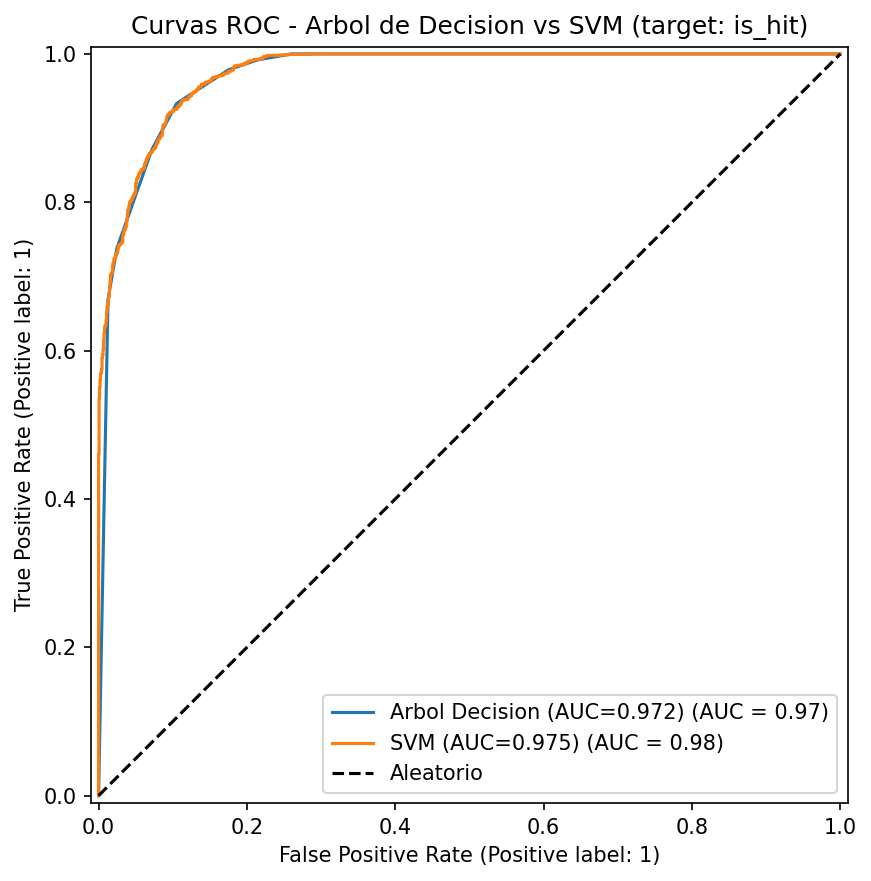
\includegraphics[width=0.82\textwidth]{figures/21_roc_comparacion.png}
\caption{Curvas ROC de los modelos de clasificaci\'on binaria. Ambos superan un \'area de 0.97, lo que indica una capacidad de discriminaci\'on alta entre t\'itulos que ser\'an hits y los que no.}
\end{figure}

% ---------------------------------------------------------------
% HITO 4 - PROTOTIPO DE VISUALIZACION
% ---------------------------------------------------------------
\newpage
\section*{Prototipo de Visualizaci\'on: Dashboard Interactivo}

El prototipo de visualizaci\'on es un dashboard desarrollado en Streamlit que integra todos los resultados del proyecto en una interfaz web interactiva. El dashboard est\'a compuesto por siete secciones, cada una orientada a responder preguntas espec\'ificas de negocio a partir de los datos y modelos entrenados.





\end{document}
